In this chapter we introduce the concepts of neutron scattering and shortly present the different types of instruments typically found at a research reactor (Sec. \ref{sec:scattering}). A special emphasis is put on triple-axis spectrometers (TAS) as the work-horse of inelastic scattering (Sec. \ref{sec:scattering}). Finally, we summarise the current state of autonomous experimentation (Sec. \ref{sec:autonomous}).



\section{Neutron scattering \label{sec:scattering}}

The history of neutron physics begins in 1932 with the discovery of the neutron by James Chadwick, who used alpha particles (helium nuclei) to bombard a beryllium-9 sample, thereby producing carbon-12 and one neutron per reaction \cite[p.1]{Jacrot2021}. The neutron was found to have a similar mass as the proton ($m_n = 1.675\cdot10^{-27}\,\mathrm{kg}$, $m_p = 1.673\cdot10^{-27}\,\mathrm{kg}$), but, as the name implies, does not possess a charge \cite[p. 2]{Squires2012}. The absence of a charge makes the neutron very useful for science, as it is subject to purely nuclear interactions with other nuclei, without any electrostatic repulsion \cite[p. 1]{Squires2012}.

In 1939, Otto Hahn used a Chadwick-type neutron source to irradiate uranium isotopes in an attempt to produce heavy trans-uranium elements \cite{wiki_fission}. But instead of heavier elements, the experiment yielded lighter elements, which was interpreted by Lise Meitner as a splitting of the uranium nucleus, the discovery of nuclear fission \cite{wiki_fission}. A typical possible channel of a fission reaction is the decay of uranium-235 into baryum-144 and krypton-89, where two to three neutrons are produced by each reaction in addition to the daughter nuclei and energy \cite{wiki_fission}.

In 1942, Enrico Fermi made use of the excess neutrons that are obtained by each fission reaction to produce a continuous, self-sustaining chain reaction in the first artificial nuclear reactor, the \textit{Chicago Pile-1}~\cite[p.1]{Jacrot2021}~\footnote{Note that \textit{Chicago Pile-1} was the first \textit{artificial} nuclear reactor. The first \textit{natural} reactor was discovered to have run more that 1.5 billion years ago in Oklo, Gabun, at an average power of about 100 kW for a period of half a million years \cite{wiki_oklo}.}.

The first research reactor, having a power of 3.5 MW~\footnote{As research reactors do not produce electricity, the given numbers refer to thermal powers.} and being used for studies in solid-state physics, was built in Oak Ridge, USA in 1943, shortly after Fermi's pile \cite[p.3]{Jacrot2021}. 
Here, first neutron scattering experiments were performed by Clifford Shull using a two-axis diffractometer \cite[p.3]{Jacrot2021}.

A two-axis diffractometer is used for studying the structure of crystals. This is possible, because neutrons coming from the reactor can be slowed down (moderated) into energy regions where their de Broglie wavelength $\lambda = h/p$ corresponds to typical inter-atomic distances in crystal unit cells, which is of the order of 1 \AA{}ngstr\"om, i.e. $10^{-10}$ m \cite[pp.1,3]{Squires2012}.



\section{Triple-axis spectrometers \label{sec:tas}}

The triple-axis spectrometer (TAS) is one of the fundamental types of instruments in the field of neutron scattering at research reactors.

\clearpage
\begin{figure*}[htb]
	\centering
	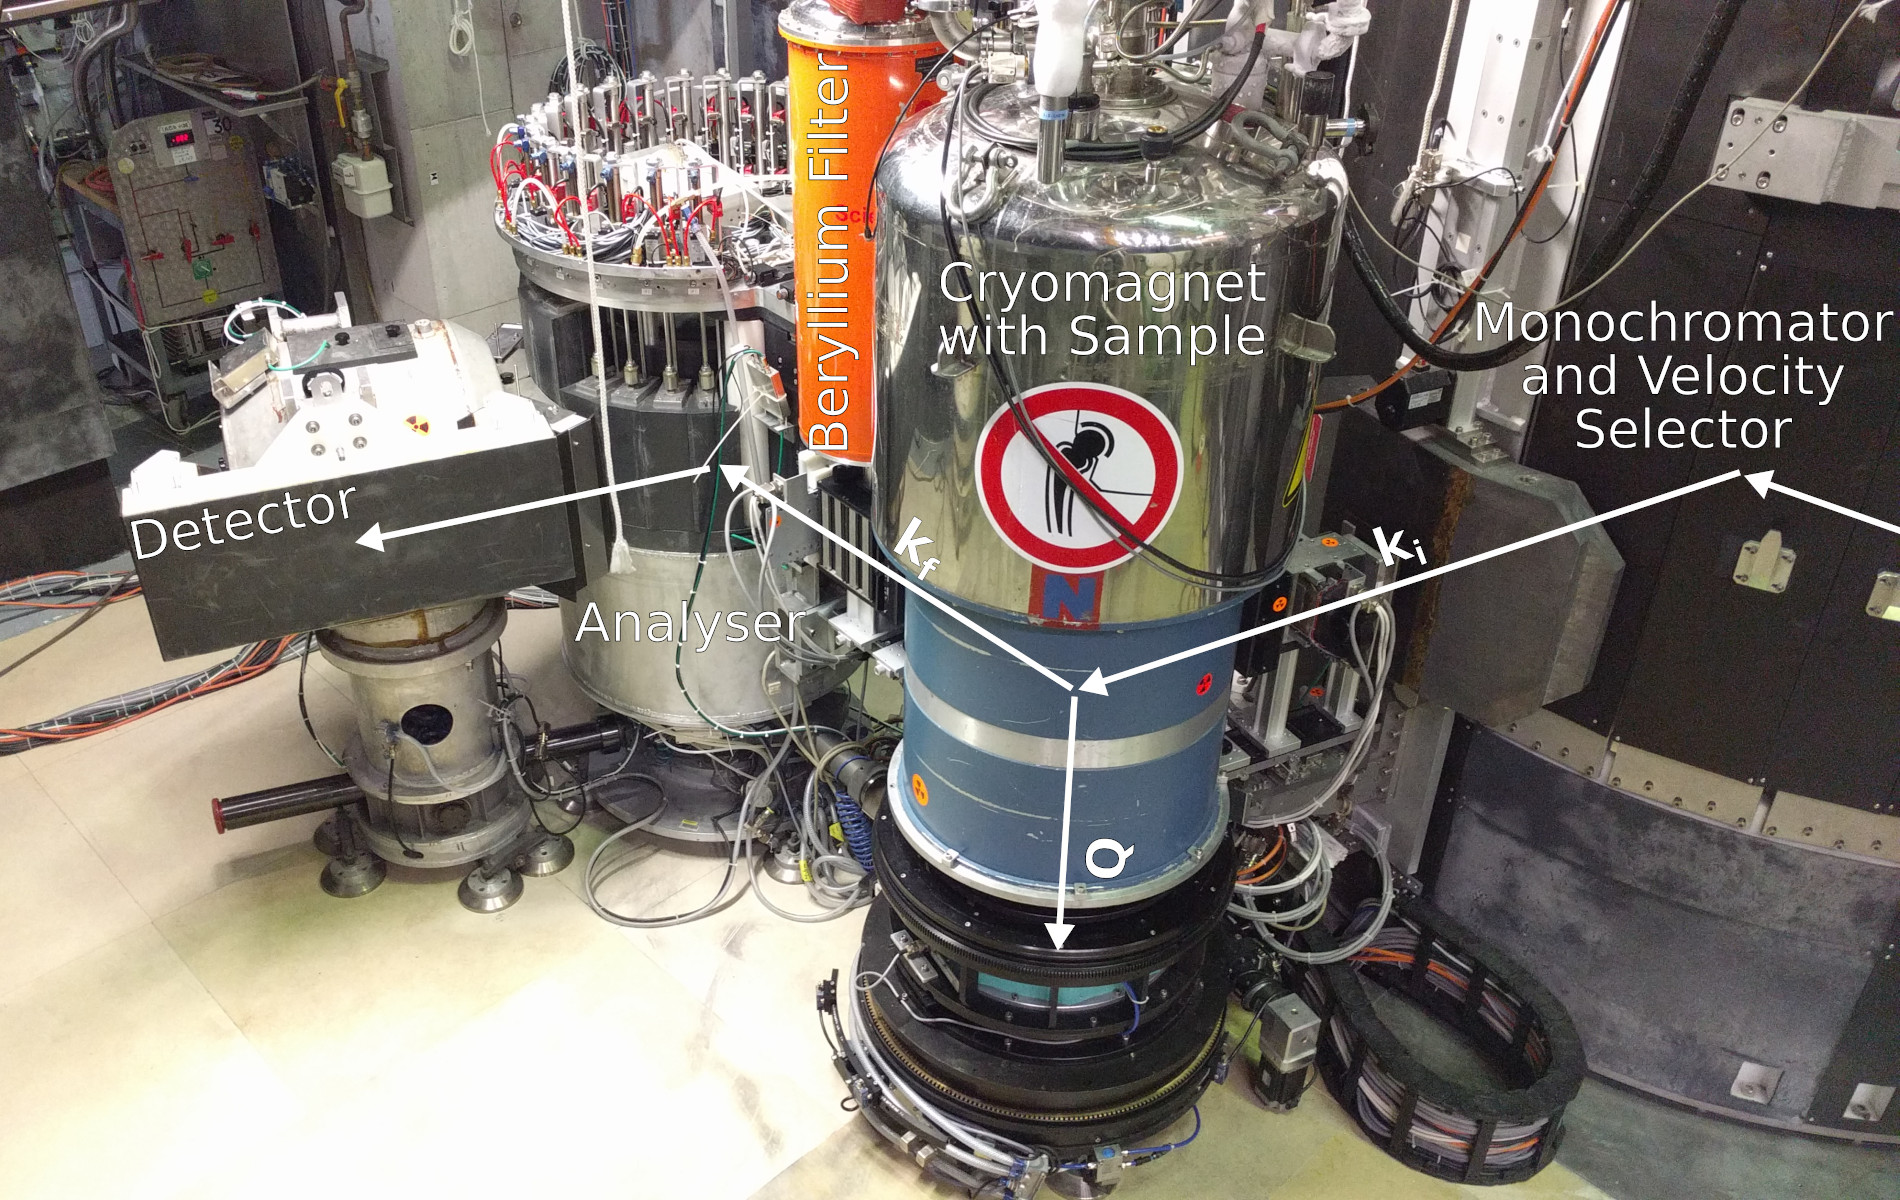
\includegraphics[width=0.75\textwidth]{figures/thales.jpg}
	\caption{The triple-axis spectrometer ThALES \cite{thales} at the Institut Laue-Langevin in Grenoble, France. This picture is reproduced from \cite{TODO}.}
	\label{fig:thales}
\end{figure*}



\section{Autonomous experiments \label{sec:autonomous}}

The goal of this work is the design and implementation of software tools which enable an automatic path finding for TAS instruments.
Automatic path finding is necessary for the instrument to circumvent obstacles in its path. The methods in this work are part of the current drive towards autonomous experimentation.
